\section{Проектування програмного продукту}
\subsection{Концептуальне проектування}
\noindent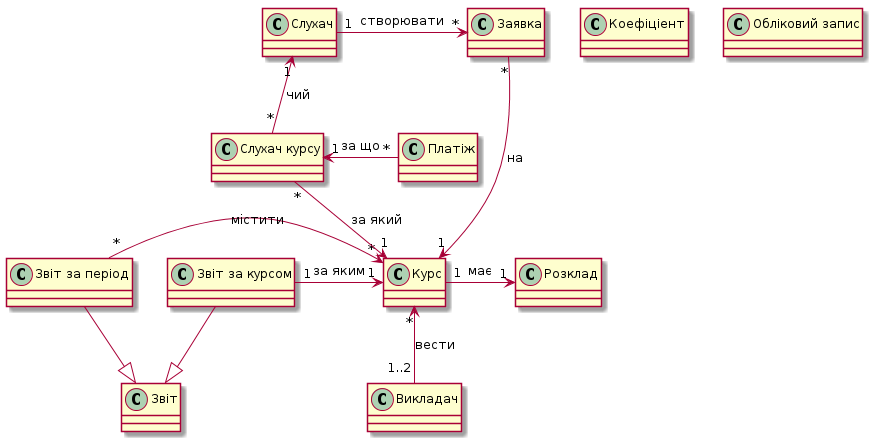
\includegraphics[width=17cm]{pp_pw3_conc.png}
\imglabel{Діаграма концептуальних класів}
\subsection{Логічне проектування}
\noindent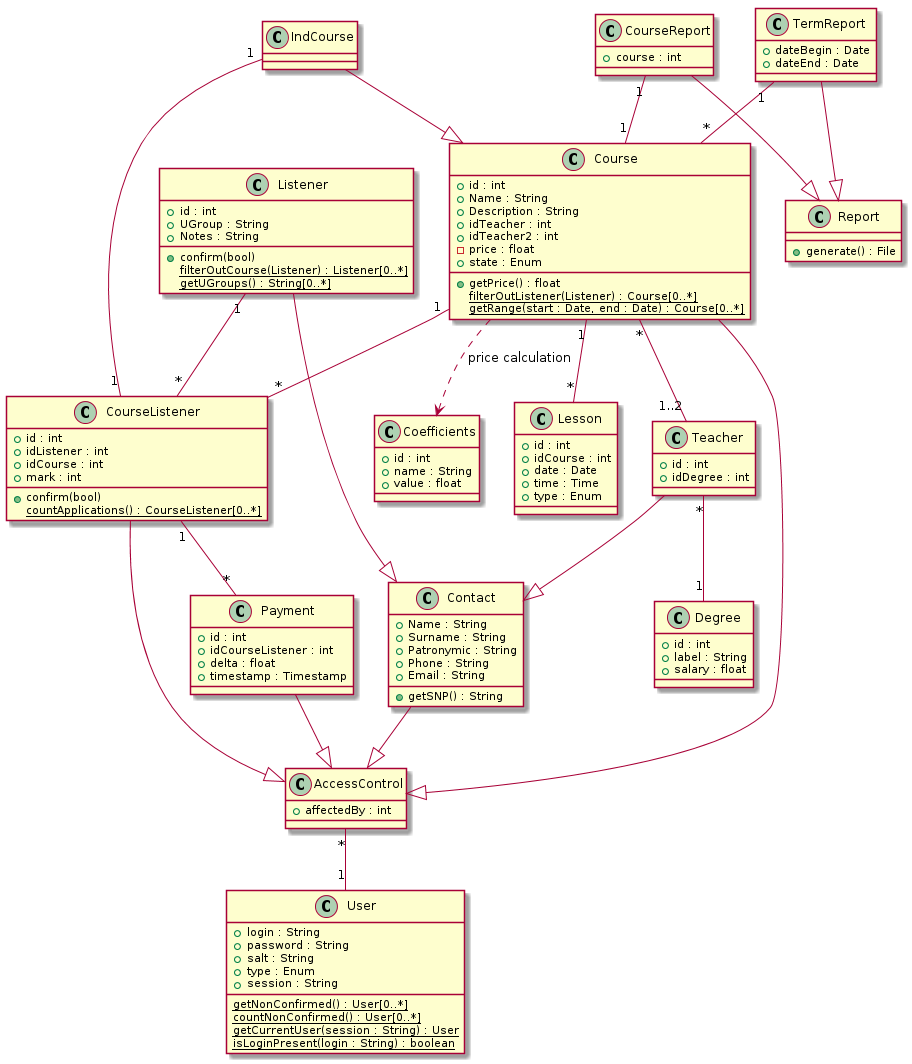
\includegraphics[width=17cm]{pp_pw3_clas.png}
\imglabel{Діаграма програмних класів}

\newpage
\subsection{База даних}
\def\dbtable#1#2#3{
 \tablabel{Опис структури таблиці "#1" (#2)}
 \begin{supertabular}{|p{1.2cm}|p{3.5cm}|p{3cm}|p{2.6cm}|p{1.2cm}|p{3.3cm}|}
 \hline
 Ключ & Назва & Ім'я поля & Тип & NULL & Дод.\\
 \hline
 #3
 \hline
 \end{supertabular}
}
\newcommand{\tabheader}[2]{
 #1 \emph{(#2)}
}
\dbtable{Слухачі}{listeners}{
PK & Ідентифікатор & idListener & int(6) & Ні & A\_I\\
 & Ім'я & Name & varchar(30) & Так & \\
 & Прізвіще & Surname & varchar(30) & Ні & \\
 & По батькові & Patronymic & varchar(30) & Так & \\
 & Університетська група & UGroup & varchar(6) & Так & \\
 & Телефон & Phone & varchar(20) & Так & \\
 & E-mail & Email & varchar(40) & Так & \\
FK & Ким змінено & affectedBy & varchar(32) & Ні & \\
}
\dbtable{Курси}{courses}{
PK & Ідентифікатор & idCourse & int(6) & Ні & A\_I\\
 & Назва & Name & varchar(50) & Ні & \\
 & Опис & Description & varchar(400) & Так & \\
 & Ознака індивідуального курсу & isIndividual & bit(1) & Ні & \\
FK & Викладач & idTeacher & int(6) & Так & \\
FK & Другий викладач & idTeacher2 & int(6) & Так & \\
 & Ціна & Price & decimal(10,2) & Так & \\
 & Кількість годин & hours & smallint(3) & Ні & \\
 & Стан & state & tinyint(1) & Ні & 0..2 (Йде набір, набрано, завершений)\\
FK & Ким змінено & affectedBy & int(6) & Ні & \\
}
\dbtable{Слухачі курсу}{Course\_Listeners}{
PK & Ідентифікатор & idCL & int(6) & Ні & A\_I\\
FK & Курс & idCourse & int(6) & Ні & \\
FK & Слухач & idListener & int(6) & Ні & \\
 & Оцінка & mark & tinyint(3) & Так & \\
FK & Ким змінено & affectedBy & int(6) & Ні & \\
}
\newpage
\dbtable{Платежі}{payments}{
PK & Ідентифікатор & idPayment & int(6) & Ні & A\_I\\
FK & Слухач курсу & idCL & int(6) & Ні & \\
 & Кошти & delta & int(6) & Ні & \\
 & Мітка часу & timestamp & timestamp & Ні & CURRENT\_\ TIMESTAMP\\
}
\dbtable{Викладачі}{teachers}{
PK & Ідентифікатор & idTeacher & int(6) & Ні & A\_I\\
 & Ім'я & Name & varchar(30) & Так & \\
 & Прізвіще & Surname & varchar(30) & Ні & \\
 & По батькові & Patronymic & varchar(30) & Так & \\
 & Телефон & Phone & varchar(20) & Так & \\
 & E-mail & Email & varchar(40) & Так & \\
FK & Ким змінено & affectedBy & varchar(32) & Ні & \\
FK & Вчений ступінь & degree & tinyint(2) & Так & \\
}
\dbtable{Розцінки}{prices}{
PK & Ідентифікатор & degree & tinyint(2) & Ні & A\_I\\
 & Вчений ступінь & deglab & varchar(30) & Ні & \\
 & Зарплата & salary & decimal(10,2) & Ні & \\
}
\dbtable{Коефіціенти}{coefficients}{
PK & Ідентифікатор & idCoefficient & tinyint(2) & Ні & A\_I\\
 & Мітка & name & varchar(128) & Так & \\
 & Значення & value & float & Так & \\
}
\newpage
\dbtable{Користувачі}{users}{
PK & Логін & login & varchar(32) & Ні & \\
 & Хеш паролю & password & text & Ні & \\
 & Сіль & salt & text & Ні & \\
 & Тип & isAdmin & tinyint(1) & Ні & 0..2 (Оператор, Адміністратор, Переглядач)\\
 & Ключ сесії & sessionid & text & Так & \\
}
